In this chapter, the loading procedure and unloading procedure will be explain. The loading procedure is related to the workcell, which means that LEGO bricks are moved from the mobile robot to the workcell. The unloading procedure is the opposite, i.e. LEGO bricks are moved from the workcell to the mobile robots.

\section{Loading LEGO bricks to workcell procedure}
The workcell will receive an order message from the MES server. It will activate the conveyer belt and then wait for a lego brick to be detected, by the vision system. If the vision system detects a LEGO brick the workcell robot will move to the LEGO brick and grasp it. The information used for the grasping is position, orientation and velocity acquired from the vision system and the vision velocity feedback respectively. The workcell robot then moves to either the order box or the leftover box, depending upon the LEGO brick. It will then ungrasp the LEGO brick. This will continue until the order is complete. A message will then inform the MES server that the order has been fulfilled. A block diagram of this process can be observed in figure \ref{fig:overall_block_diagram_loading}.

\begin{figure}[ht]
\centering
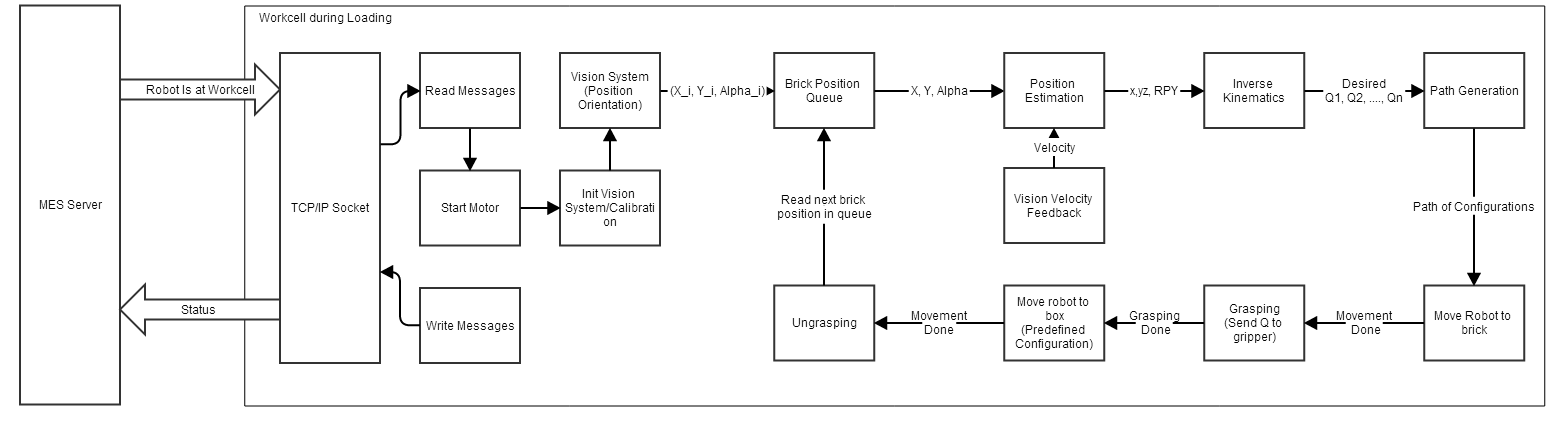
\includegraphics[width=\textwidth]{images/overall_block_diagram_loading.png}
\caption{Diagram illustration the loading procedure}
\label{fig:overall_block_diagram_loading}
\end{figure}


\section{Unloading LEGO bricks to mobile robot procedure}
When the workcell robot has finished sorting the LEGO bricks, a message to the MES will be sent. When a mobile robot has arrived at the end of the conveyor belt the workcell robot will then move to a predefined position for grasping the boxes of lego bricks. While holding the LEGO box the workcell robot now moves the box to the conveyor belt and places it in a predefined position on the belt. The conveyor belt then moves the box to the waiting mobile robot and after a certain amount of time, the belt is stopped. It will then be considered if new boxes are need for further work. The workcell robot then returns to its loading state and send a message to the MES server indicating it is ready for a new order. A block diagram of this process can be observed in figure \ref{fig:overall_block_diagram_unloading}.

\begin{figure}[ht]
\centering
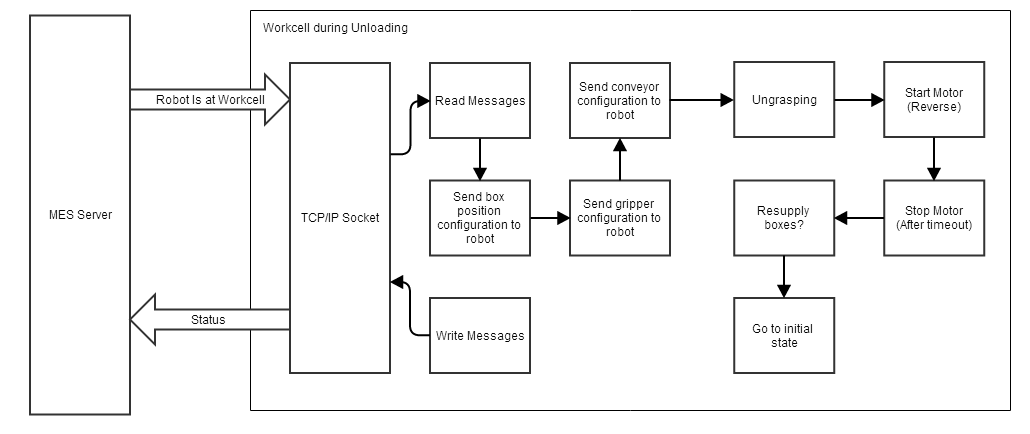
\includegraphics[width=\textwidth]{images/overall_block_diagram_unloading.png}
\caption{Diagram illustration the unloading procedure}
\label{fig:overall_block_diagram_unloading}
\end{figure}